\title{\pkg{reclin2}: a Toolkit for Record Linkage and Deduplication}
\author{by D. Jan van der Laan} 
\maketitle

\abstract{
The goal of record linkage and deduplication is to detect which records belong to the same object in
data sets where the identifiers of the objects contain errors and missing values.  The main design
considerations of \pkg{reclin2} are: modularity/flexibility, speed and the ability to handle large
data sets.  The first points makes it easy for users to extend the package with custom process
steps. This flexibility is obtained by using simple data structures and by following as close as
possible common interfaces in R. For large problems it is possible to distribute the work over
multiple worker nodes.  A benchmark comparison to other record linkage packages for R, shows that
for this specific benchmark, the \pkg{fastLink} package performs best. However, this package only
performs one specific type of record linkage model. The performance of \pkg{reclin2} is not far
behind the of \pkg{fastLink} while allowing for much greater flexibility. 
}

% =============================================================================
% =============================================================================
\section{Introduction}

Combining different data sets is often an important step in many data analysis projects. Sometimes
the data sets will contain high quality linkage keys, especially when the data sets are based on a
common register. For example, the samples for (nearly) all social surveys performed at Statistics
Netherlands are drawn from the population register and therefore can be linked to each other
\citep{ssb}. In these cases exact linkage can be used. In exact linkage, records are linked when
they agree exactly on the linkage keys used. Exact linkage can be performed in R using
base functions such as \code{merge}.  However, it is not uncommon that data sets have to be linked
on keys such as `first name', `last name' and `address`. Often these variables contain errors and/or
missing values and, therefore, exact linkage is not possible. That is where probabilistic record
linkage methods come into play \citep{herzog,datamatching}.  These methods will calculate some sort
of likelihood that two records belong to the same object (person, company, \ldots). This will be
called a match. Only record pairs with a high enough likelihood are linked to each other.  The goal
is to minimise the number of false links (linking two records that do not belong to the same object)
and the number of missed links (\emph{not} linking two records that do belong to the same object).

The process of probabilistic record linkage generally consists of the following steps: (1) Generate
pairs of records from each of the two data sets that are to be linked; (2) Compare the two records
of the pair and generate a comparison vector (in the simplest case this a vector of ones and zeros
coding agreement/disagreement on each of linkage keys); (3) Estimate a model that predicts based on
the comparison vector a likelihood that the two records belong to the same object; (4) Select pairs
with a high enough likelihood; (5) Using the selected pairs, generate the final linked dataset. 
\pkg{reclin2} offers different methods for most of these steps and by mixing the different methods a
custom linkage process can be developed. This is discussed in more detail with examples in the
section on the record linkage process.

A variant of record linkage is deduplication. Here there is only one data set and one wants to
determine which records belong to the same object. For example, a customer database can contain the
same customer multiple times with slightly different information (e.g. different email addresses).
Deduplication is usually performed by linking a dataset to itself. Matches are then duplicate
records. The principles are, therefore, the same as with regular record linkage and in the remainder
of paper we will focus on regular record linkage of two data sets. 

Record linkage can be computationally and memory intensive. In principle each record from a data
set has to be compared to each record in the other data set. Therefore, when the two data sets are
of size $N_1$ and $N_2$ respectively the computational complexity and memory requirements are of
order $O(N_1 N_2)$. For example, at Statistics Netherlands one common data set is the population
register containing in the order of $10^7$ records; other data sets  can be in the order of
$10^3$--$10^5$, resulting in $10^{10}$-$10^{12}$ possible comparisons.

\CRANpkg{reclin2} is a package that provides a set of tools to perform probabilistic record linkage. It
is the successor of the \CRANpkg{reclin} package. The reason for the update was to be able to provide
better support for the core design considerations of the \pkg{reclin}/\pkg{reclin2} package.
Unfortunately this was not possible while keeping backward compatibility, therefore it was decided
to continue with a new package. The core design considerations are:
\begin{enumerate}
  \item Modularity/flexibility.
  \item Speed.
  \item Ability to handle large datasets. 
\end{enumerate}
The last two points are important because of the aforementioned issues with the size of the
problem. The first point is important, as in practice no record linkage project is the same and,
therefore, a common need is to vary on the default procedure.  The next section will discuss how
we tried to address the points above. Besides \pkg{reclin2} other packages exist for
probabilistic record linkage. There is the \CRANpkg{RecordLinkage} \citep{RecordLinkage}
package that implements various methods such as classic probabilistic record linkage based on the
\citet{fs} model and methods based on machine learning. Furthermore, there is the \CRANpkg{fastLink}
\citep{fastlink, fastlink2} package that focuses on a fast and flexible implementation of the
Fellegi-Sunter model. The main difference of \pkg{reclin2} with these packages is the focus on the
previous three points: \pkg{fastLink} scores well on points 2 and 3, but only supports one type of
model while \pkg{RecordLinkage} scores well on point 3 and better than \pkg{fastLink} on point 1,
but lacks some flexibility and speed. Points 2 and 3 are investigated in a later section using a
benchmark.

% =============================================================================
% =============================================================================
\section{Design considerations}

One of the main considerations when designing the package was flexibility. Therefore, the package
has been designed as a set of functions that operate on \CRANpkg{data.table} objects
\citep{datatable}. The main object of the package is the \code{pairs} object which is a subclass of
\code{data.table}. The \code{pairs} object contains pairs of records from the two datasets that are
to be linked (called \code{x} and \code{y}). The first two columns of the \code{pairs} object
contain the indices of the corresponding records from the two data sets.  Most functions of the
package accept a \code{pairs} object and return a \code{pairs} object. The package has functions for
different steps in the linkage process (as described in the next section).  By combining the
different available functions a custom data linkage process can be built. Furthermore, as the
\code{pairs} object is a \code{data.table} it is also easy for the user to manipulate it. For
example, new columns can be derived and pairs can be filtered. Functions that do not manipulate the
\code{pairs} object are designed to follow as closely as possible the common interfaces of base R
functions. For example, the function \code{problink\_em} that can be used to estimate the parameters
of the Fellegi-Sunter model accepts similar input as other modelling functions in R: e.g. a formula
to specify the model and a \code{data} argument to pass in the data on which to estimate the model.
The corresponding \code{predict} function can be used to calculate likelihoods for pairs being a
match.  It is therefore also easy to use models from other packages, such as machine learning
methods, to estimate the likelihoods.  Where a package such as \pkg{RecordLinkage} has functions for
a number of machine learning methods, \pkg{reclin2} does not need these as the user is free to call
these themselves as demonstrated in the section on the record linkage process below. 

The other two design considerations, speed and being able to handle large datasets, are obtained in
two ways. First, by using a \code{data.table} as the main object. Most methods have an
\code{inplace} argument (default value is \code{FALSE}). When set to \code{TRUE} the \code{pairs} object
is modified using the \code{[, :=]} operation of a \code{data.table}. This prevents unnecessary copies,
decreasing memory consumption and increasing speed. Second, there is the option to create a cluster
and distribute the computational load over multiple cores. 
Using functionality from the \pkg{parallel} or \CRANpkg{snow} \citep{snow}
packages, multiple R processes are started and the data is distributed over these processes. Each
process then generates a subset of the pairs which are kept within the process. Subsequent
operations on the pairs, such as comparison, are also distributed over the processes where each
process applies the operation to its subset of pairs.  One of the more computationally intensive
operations during linkage is comparing the records from the two data sets to each other. This
problem scales well when parallelising.  Therefore parallelization can lead to a significant speed
up. Furthermore, when using a \CRANpkg{snow} cluster the computation can also be distributed over
multiple machines. This can not only lead to a speed up, but also means that the memory of multiple
machines can be utilized allowing for larger problems than could be handled on a single machine.  To
work with a cluster, special functions with the \code{cluster\_} prefix are offered. The cluster
functions generating the pairs expect as on of their inputs a valid cluster created for example
using \code{makeCluster} from the \pkg{parallel} package.  When using the cluster variant, the
object is no longer a \code{data.table} and it becomes more difficult to manually manipulate the
object. The package has a few functions to help with this which will be discussed at the end of the
next section.



% =============================================================================
% =============================================================================
\section{The record linkage process}

This section section will give an overview of the linkage process and show how the functions in 
\pkg{reclin2} can be used for this. The discussion will be brief. An overview of the main steps of a
record linkage process has already been given in the introduction section of the paper. 
A more extensive description can be found in the package vignettes and documentation. Also, we will not
go into detail into the methods used as these are well described in, for example, \citet{herzog} and
\citet{datamatching}. 

\subsection{Generating pairs}

The first step in the linkage process is to generate pairs of records from the two data sets
\code{x} and \code{y}. There are a number of functions for this: the function \code{pair} generates
all possible pairs. However, this can lead to impractically large numbers of pairs. Therefore, often
methods are applied to reduce the total number of pairs. One commonly used method is blocking where
only pairs are generated that agree on some key. This, of course, only works when a good enough
quality key is available, otherwise true matches are lost.  Another method in the package,
\code{pairs\_simsum}, is to generate pairs that agree on a given number of variables (e.g. they have
to agree on either the postcode or the town name) \citep{datamatching}. In the example below we use
blocking on `postcode', e.g. pairs are only generated when they agree exactly on `postcode'
(\code{[...]} in the examples indicate removed output).

\begin{example}
> library(reclin2)
[...]
> data("linkexample1", "linkexample2")
> (pairs <- pair_blocking(linkexample1, linkexample2, "postcode"))
  First data set:  6 records
  Second data set: 5 records
  Total number of pairs: 17 pairs
  Blocking on: 'postcode'

    .x .y
 1:  1  1
 2:  1  2
 3:  1  3
 4:  2  1
 5:  2  2
 6:  2  3
 7:  3  1
[...]
\end{example}
A \code{data.table} is returned with the added class \code{pairs}. The columns \code{.x} and
\code{.y} contain the row indices into the two data sets. A copy (when the original data sets are
not modified this is only a reference) of the two data sets is stored in the attributes \code{x} and
\code{y}. This makes some of the next function calls easier. 

There also exist cluster variants of these functions that return a \code{cluster\_pairs} object:
\begin{example}
> library(parallel)
> cl <- makeCluster(2)
> cpairs <- cluster_pair_blocking(cl, linkexample1, linkexample2, "postcode")
\end{example}
When calling the cluster variants of the pair generating algorithms, the records from \code{x} are
randomly distributed over the nodes of the cluster and \code{y} is copied to each cluster node. On
each node the corresponding pair function is called. The resulting \code{pair} object is stored on
each node in an environment in the environment \code{reclin2:::reclin\_env} (the default name of
this environment is \code{"default"}).  The \code{cluster\_pairs} object is a list with a copy of
the cluster object and the name of the environment on the cluster nodes in which the pairs are
stored.


\subsection{Comparing pairs}
The next step in the linkage process is to compare the pair of records on a set of common variables
in both data sets. For this the package contains various comparison functions. The default function
checks for exact agreement. However, for text fields such as names and addresses, it often better to
allow for spelling errors. For this some of the functions from the \CRANpkg{stringdist}
\citep{stringdist} package are imported. For classic record linkage using the Fellegi-Sunter model
is necessary that these are translated into a similarity score between 0 and 1 where 1 is complete
agreement which is what the functions included in \pkg{reclin2} do. In the example below, we provide
a comparison function for `firstname', `lastname' and `address':
\begin{example}
> (compare_pairs(pairs, on = c("lastname", "firstname", "address", "sex"),
+   comparators = list(lastname = jaro_winkler(0.9), firstname = jaro_winkler(0.9),
+      address = jaro_winkler(0.9) ), inplace = TRUE))
[...]
    .x .y lastname firstname   address   sex
 1:  1  1 1.000000 0.4722222 0.9230769    NA
 2:  1  2 0.000000 0.5833333 0.8641026  TRUE
 3:  1  3 0.447619 0.4642857 0.9333333  TRUE
[...]
\end{example}
The Jaro-Winkler string similarity score is used: a value of one indicates complete agreement, 
a value of zero indicated complete disagreement (no overlap in letters) and values in between
indicate partial agreement. The \code{0.9} in the function call is a threshold used, among others, by
the EM-algorithm discussed below as this method only handles complete agreement or disagreement:
values above 0.9 are considered to agree completely.  We see that the first record from \code{x}
agrees exactly only on `lastname' with the first record of \code{y}, while `sex` cannot be compared
as it is missing in at least one of the data sets. 

The \code{compare\_pairs} method is also implemented for the \code{cluster\_pairs} object. For more
flexibility there is also the \code{compare\_vars} method. This function only compares one variable
at the time, but it allows for different names of the variables in the two data sets, generating
multiple output columns out of one comparison and for more complex comparisons where multiple
variables are taken into account. As an example of the latter, the code below compares records on
first name and last name allowing for the two parts of a name to be swapped:
\begin{example}
> comp_name <- function(x, y) {
+   equal <- identical()
+   regular <- equal(x[[1]], y[[1]]) & equal(x[[2]], y[[2]])
+   swapped <- equal(x[[1]], y[[2]]) & equal(x[[2]], y[[1]])
+   regular | swapped
+ }
> compare_vars(pairs, "name_swap", on_x = c("firstname", "lastname"),
+   comparator = comp_name)
[...]
    .x .y lastname firstname   address   sex name_swap
 1:  1  1 1.000000 0.4722222 0.9230769    NA     FALSE
 2:  1  2 0.000000 0.5833333 0.8641026  TRUE     FALSE
 3:  1  3 0.447619 0.4642857 0.9333333  TRUE     FALSE
[...]
\end{example}
When records are compared on multiple columns, the comparison function receives two
\code{data.table} objects as its inputs. 


\subsection{Scoring pairs}

The goal of probabilistic record linkage is to generate a likelihood for each pair that the two
records in the pair belong to the same record. This likelihood is based on the comparison vector.
The traditional method is the model by \citet{fs}. The parameters of this model are usually
estimated using a EM-algorithm \citep{em}. However, \pkg{reclin2} considers this just a model as any
other model and uses the same interface as any other model that can be estimated in R:

\begin{example}
> m <- problink_em(~ lastname + firstname + address + sex, data = pairs)
> (pairs <- predict(m, pairs = pairs, add = TRUE))
[...]
    .x .y lastname firstname   address   sex    weights
 1:  1  1 1.000000 0.4722222 0.9230769    NA  7.7103862
 2:  1  2 0.000000 0.5833333 0.8641026  TRUE -5.9463949
 3:  1  3 0.447619 0.4642857 0.9333333  TRUE  0.8042090
[...]
\end{example}
The range of the weights depends on the number of variables and the estimated parameters in the
model. They are log-likelihood ratios \citep{fs}. The values of the weights themselves are not
directly of use, except that a higher weight indicates that a pairs if more likely a match. In
principle, a weight above zero indicates that the pair is more likely a match than not. However, in
practice, a threshold higher than zero is often used in order to reduce the likelihood of false
links. The predict function of the EM-model also has the option to estimate posterior probabilities.
Thresholds for the weights (or probabilities) are often determined by manually inspecting pairs
around potential threshold values \citep{herzog}.  These methods can also be used for
\code{cluster\_pairs} objects. 

As the \code{pairs} object is a regular \code{data.table} object, it is also relatively easy to 
estimate other models on the data set.  In principle this is a classification problem: the pairs
need to be divided into two categories: matches and non-matches. For example, when for a part of the
pairs the true match status is known, a supervised learning method can be used. In the example below
the `id' field is used to derive the true match status for the dataset (in practice this would
probably only be available for a subset) and predict a linkage probability using logistic
regression:
\begin{example}
> compare_vars(pairs, "true", on_x = "id", on_y = "id", inplace = TRUE)
> mglm <- glm(true ~ lastname + firstname, data = pairs,
+   family = binomial())
> pairs[, pglm := predict(mglm, type = "response")]
\end{example}
In the first line of this example, a column named `true' is added to the dataset (in place).
This column is a comparison of the `id' from the first data set (\code{on\_x = "id"}) to the `id'
column of the second data set (\code{on\_y = "id"}). This column `true' contains the true match
status. In the second line, a logistic regression model is estimated that predicts the match status
using the two columns `firstname' and `lastname'. Using this model the probability of a true match
is estimated in the final line of the example and added to the data set.

\subsection{Creating the linked data set}

In order to link the pairs a suitable threshold needs to be determined for the weights. Records with
a weight above this threshold are classified as a match. Also, we generally know that each person
only has one record in each data set. So, generally we will want to enforce one-to-one linkage. This
will also generally improve the quality of the linked data set.  \pkg{reclin2} has two methods for
enforcing one-to-one linkage. The method \code{select\_n\_to\_m} tries to select the pairs in such a
way that the total weight of the selected pairs is maximised while linking each record from each
data set to at most one record from the other data set (using its arguments it is also possible to
enforce n-to-one or one-to-n linkage). A faster method that can lead to less links is
\code{select\_greedy} that will try to select the pair with the highest weight for each record.
Below the first method is applied; records with a weight below 0 are not considered (\code{threshold
= 0}):
\begin{example}
> (pairs <- select_n_to_m(pairs, "weights", variable = "select", threshold = 0))
[...]
    .x .y lastname firstname   address   sex    weights select
 1:  1  1 1.000000 0.4722222 0.9230769    NA  7.7103862  FALSE
 2:  1  2 0.000000 0.5833333 0.8641026  TRUE -5.9463949  FALSE
 3:  1  3 0.447619 0.4642857 0.9333333  TRUE  0.8042090  FALSE
 4:  2  1 1.000000 0.8888889 0.9230769    NA  8.6064218   TRUE
[...]
\end{example}
The method creates a logical column (name given by the `variable' argument) in the pairs object with
the selected pairs.  The first pair has a high enough weight to be selected, but there is another
candidate for the first record of \code{y} that is more likely, namely record 2 from \code{x} (see
fourth row of the output above).

Up until now we are still working with a set of pairs. The goal is to get an actually linked dataset
containing matched records from both data sets. This can be done using the \code{link} method. This
function takes the pairs and the name of a logical column indicating which pairs are selected and it
will generate the final linked data set. The output is similar to that of \code{merge}. The method
also has arguments \code{all\_x} and \code{all\_y} that function the same as the corresponding
\code{all.x} and \code{all.y} arguments of \code{merge}.
\begin{example}
> (linked_data_set <- link(pairs, selection = "select"))
  Total number of pairs: 4 pairs

   .y .x id.x lastname.x firstname.x  address.x sex.x postcode.x id.y
1:  1  2    2      Smith      George 12 Mainstr     M    1234 AB    2
2:  2  3    3    Johnson        Anna 61 Mainstr     F    1234 AB    3
3:  3  4    4    Johnson     Charles 61 Mainstr     M    1234 AB    4
4:  4  6    6   Schwartz         Ben  1 Eaststr     M    6789 XY    6
   lastname.y firstname.y     address.y sex.y postcode.y
1:      Smith      Gearge 12 Mainstreet  <NA>    1234 AB
2:     Jonson          A. 61 Mainstreet     F    1234 AB
3:    Johnson     Charles    61 Mainstr     F    1234 AB
4:   Schwartz         Ben        1 Main     M    6789 XY
\end{example}

For the \code{cluster\_pairs} the steps above need to change a little bit as \code{select\_n\_to\_m}
needs to consider all pairs and, therefore, does not work with objects of type \code{cluster\_pair}
where the pairs are distributed over the cluster nodes.
Therefore, we first need to copy the relevant pairs to the main R process. We can use a selection
variable for this only returning the pairs with a weight above zero:
\begin{example}
> cpairs <- predict(m, pairs = cpairs, add = TRUE)
> select_threshold(cpairs, "weights", variable = "initial", threshold = 0)
> local_cpairs <- cluster_collect(cpairs, "initial")
> local_cpairs <- select_n_to_m(local_cpairs, "weights", variable = "select")
\end{example}
The first line calculates weights for the \code{cpairs} object. In the second line a logical column
`initial' is created which is \code{TRUE} for records with a weight higher than 0. Using
\code{cluster\_collect}, we collect the pairs from the worker processes into the main R process.
Using the second argument we only collect pairs for which the column `initial' is \code{TRUE}. The
\code{local\_cpairs} object is a regular \code{pairs} object (and, therefore, also a
\code{data.table}) on which we can use the regular \code{select\_n\_to\_m} method. 


\subsection{Helper functions for \code{cluster\_pair} objects}

It is easy to do manual manipulations on the regular \code{pairs} object. For the
\code{cluster\_pairs} the \code{pairs} are distributed over the worker nodes. There are a couple of
functions to help with this. The already mentioned \code{cluster\_collect} function copies the pairs
locally. The \code{cluster\_call} function accepts the \code{cluster\_pairs} and a function. It will
call the function on each node and pass it the \code{pairs}, \code{x} and \code{y}. The results of
the functions are copied back locally. For example to get the number of pairs on each node:
\begin{example}
> unlist(cluster_call(cpairs, \(p, ...) nrow(p)))
[1] 9 8
\end{example}

The \code{cluster\_modify\_pairs} function can be used to modify the pairs. The arguments are the
\code{cluster\_pairs} and a function with the same arguments as for \code{cluster\_call}. The result
of that function overwrites the pairs object on the worker node (except when \code{NULL}). In the
example below, this is used to remove pairs with a weight of zero or lower.
\begin{example}
> (cluster_modify_pairs(cpairs, \(p, ...) p[weights > 0, ]))
  Cluster 'default' with size: 2
  First data set:  6 records
  Second data set: 5 records
  Total number of pairs: 15 pairs
  Blocking on: 'postcode'

Showing a random selection of pairs:
    .x .y lastname firstname   address   sex    weights initial
 1:  3  1 0.447619 0.4722222 0.8641026    NA  0.6017106    TRUE
 2:  4  3 1.000000 1.0000000 1.0000000 FALSE 15.4915816    TRUE
[...]
\end{example}
Note, that the original \code{cpairs} object has been modified. Using the \code{new\_name} argument
it is also possible to generate a new set of pairs.


% =============================================================================
% =============================================================================
\section{Benchmark}

In this section the performance of the packages for data linkage will be investigated using example
data from the Eurostat financed ESSnet (European Statistical System Centres and Networks of
Excellence) project on Data Integration \citep{onsdata}. The two data sets `PDR' and `CIS' were
linked to each other. The datasets have 24,750 and 24,613 records respectively resulting in
612,562,500 possible pairs when linking the complete data sets. To study the effect of the size of
the problem on the performance, samples were drawn from the two data sets based on the postcode
where care was taken to sample the same postcodes in the two datasets. The sample fraction was
varied from 0.1 to 1.0 in steps of 0.1. 

\begin{figure}[p]
  \centering
  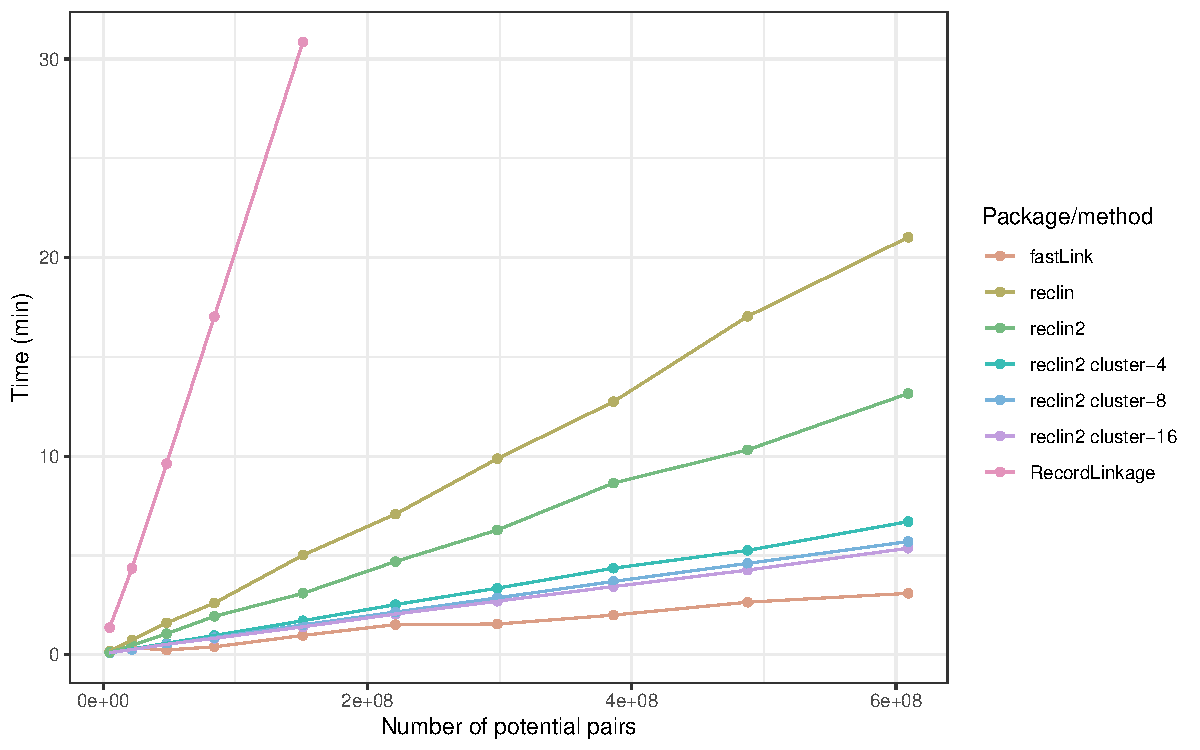
\includegraphics[width=0.9\textwidth]{benchmark_time}
  \caption{Comparison of computation times (in minutes) for the different packages (lines) as
  function of the number of potential pairs (the product of the sizes of the two data sets).  For
  \pkg{reclin2} also different numbers of worker nodes were investigated; these are denoted by
  `cluster' and the number of worker nodes. }
  \label{fig:benchtime}
\end{figure}

\begin{figure}[p]
  \centering
  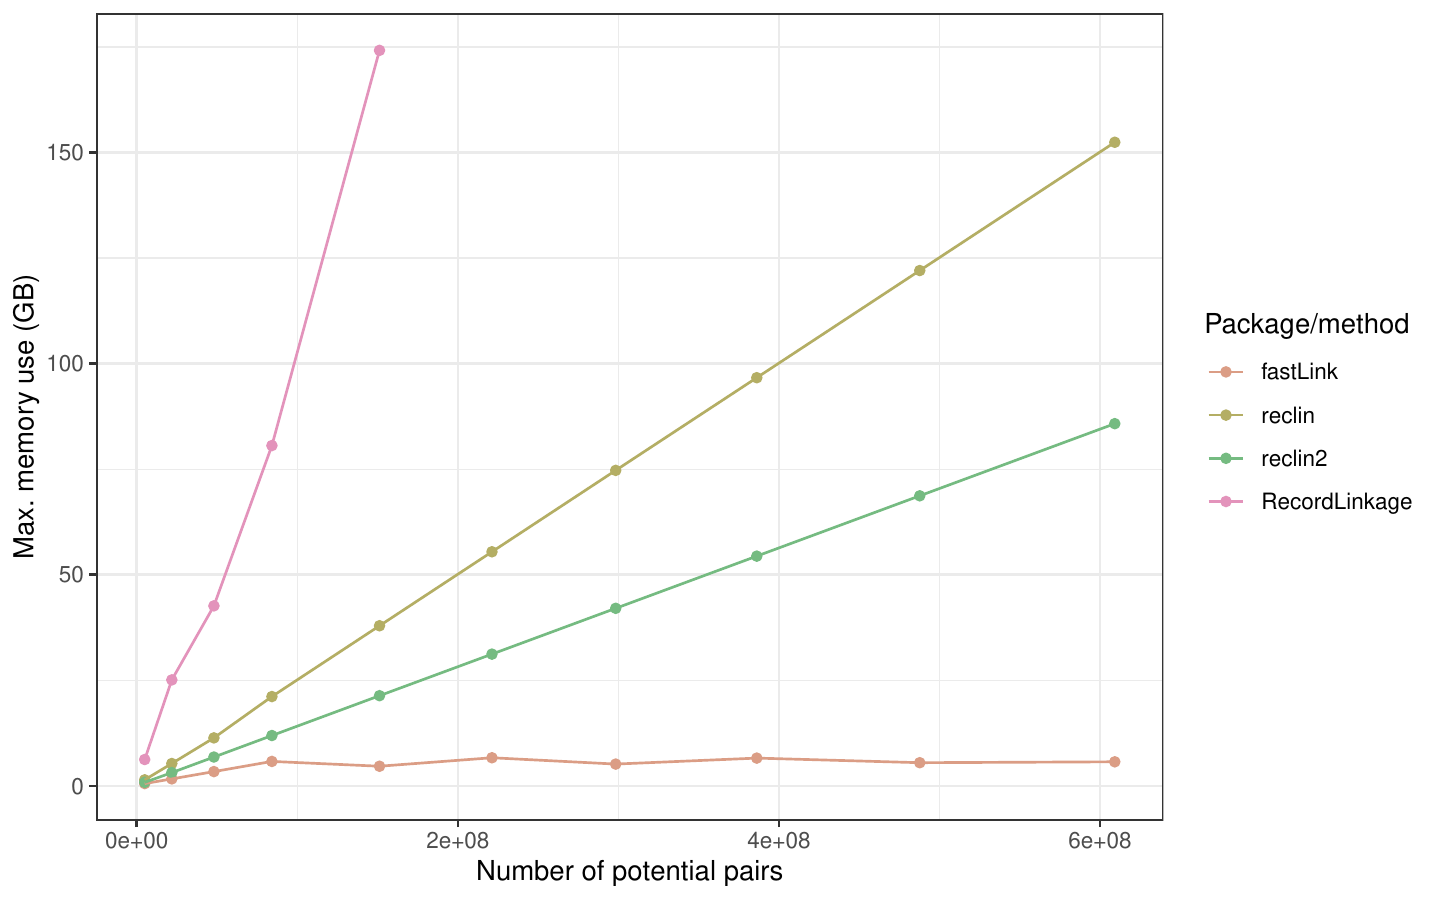
\includegraphics[width=0.9\textwidth]{benchmark_memory}
  \caption{Comparison of memory usage (in gigabytes) for the different packages (lines) as function
  of the number of potential pairs (the product of the sizes of the two data sets).  For
  \pkg{reclin2} no reliable estimates could be obtained for the runs with multiple workers.
  Therefore results are only presented for the single threaded version of \pkg{reclin2}. In
  principle the memory usage should not depend on the number of workers.}
  \label{fig:benchmem}
\end{figure}

The methods are compared on total computation time and memory use.  These were measured using the
`time` program on a Linux server. The virtual server has 16 3.2GHz Intel Xeon Gold 6146 cores and
512GB of memory and runs on Ubuntu 20.04. For the time the reported `elapsed (wall clock) time' is
used and for the memory usage the `maximum resident set size'. For \pkg{reclin2} also the effect of
different numbers of worker nodes was investigated using the cluster functions. It was attempted to
keep the methods used a close as possible to each other. No blocking was applied. The EM-algorithm
was used. For comparing the names the Jaro-Winkler similarity score was used with a threshold of
0.85. The quality of the resulting record linkage was recorded, but as the methods were not
optimally tuned, it is difficult to compare these results and these results are, therefore, not
reported. The complete code for the benchmark and all results can be found on Github
\citep{benchmark}.

Figures~\ref{fig:benchtime} and~\ref{fig:benchmem} show the computation times and the memory usage
respectively as a function of the size of the problem. For the \pkg{RecordLinkage} package larger
problem sizes than reported here were not investigated as the system started running out of memory.
\pkg{RecordLinkage} has the option to also work from disk for large problems. The performance of
this was not investigated as this would only lead to longer computation times which were already
longer than those of the other packages. For this specific problem the \pkg{fastLink} package
performs better than the other packages. Especially the memory usage is substantially lower because
of their use of specialised data structures \citep{fastlink2}. The
difference in computation time between \pkg{fastLink} and \pkg{reclin2} using multiple cores is
limited (approx. factor 1.7 for the largest problem).  However, \pkg{fastLink} is tailored for use
with the EM-algorithm while the other packages are more general. 

The speed-up of the \pkg{reclin2} benchmark is not proportional to the number of cores used. This is
caused mainly by the fact that some of the steps take place in the main process: reading and
sampling the data, starting the worker nodes, and importantly, finalizing the record linkage using
one-to-one matching. We are unfortunately limited by Amdal's law \citep{amdahl} although the
generation, comparison and (in case of the EM-algorithm) tabulation of pair and calculating the
predictions will take an increasingly larger part of the running time as the size of problem
increases.

% =============================================================================
% =============================================================================
\section{Conclusion}

By using simple data structures, namely \code{data.table} objects, and providing a set of functions
that operate on these structures, we have built a flexible and well performing toolkit for record
linkage. For users, it is easy to extend on the methods present in the package. Either by
manipulating the data structures directly, by writing custom functions or by using existing
functions. An example of the latter, is the relative ease with which existing machine learning
methods can be used in the record linkage process. 

The package manages to keep memory use limited and on machines with 256GB of memory it should handle
problems up to approximately $10^9$ pairs. By combining the memory of multiple machines this can of
course be extended. When one is only interested in using the Fellegi-Sunter model of record linkage
with an EM-algorithm to estimate the parameters of that model, the \pkg{fastLink} package is
probably the best choice. It performs better and the model and EM-algorithm used is more flexible
than that currently present in \pkg{reclin2}. The main advantage of \pkg{reclin2} over
\pkg{fastLink} is the flexibility \pkg{reclin2} provides. Especially for non standard problems this
is important. 

The package is still being developed. One of the things that is being worked on is the option
to take into account the uniqueness of a certain attribute. For example, agreement on a rare family
name is a stronger indication of a match than agreement on a common family name. However, we hope
that making it easy for users to extend and modify the record linkage processes also lowers the
threshold for contributing to the package. 

\bibliography{vanderlaan}

\address{D. Jan van der Laan\\
  Statistics Netherlands (CBS)\\
  Henri Faasdreef 313, The Hague\\
  The Netherlands\\
  ORCiD: 0000-0002-0693-1514\\
  \email{dj.vanderlaan@cbs.nl}}

